\documentclass{beamer}
\usepackage[french]{babel}
\usepackage{hyperref}
\definecolor{links}{HTML}{2A1B81}
\hypersetup{colorlinks,linkcolor=,urlcolor=links}
\usepackage{graphicx}
\usepackage{amsmath,amssymb}
\usepackage{tabularx}
\usepackage{booktabs}
\usepackage[compatibility=false]{caption}
\usepackage[toc,page]{appendix}
\usepackage{minted}
\usepackage{xspace}

\makeatletter
  \def\beamer@calltheme#1#2#3{%
    \def\beamer@themelist{#2}
    \@for\beamer@themename:=\beamer@themelist\do
    {\usepackage[{#1}]{\beamer@themelocation/#3\beamer@themename}}}

  \def\usefolder#1{
    \def\beamer@themelocation{#1}
  }
  \def\beamer@themelocation{}

\patchcmd{\minted@colorbg}{\noindent}{\medskip\noindent}{}{}
\apptocmd{\endminted@colorbg}{\par\medskip}{}{}
\makeatother

\newcolumntype{Y}{>{\centering\arraybackslash}X}

\usefolder{../theme}
\usetheme[numbering=fraction,block=fill,progressbar=frametitle]{metropolis} %Use metropolis theme

\definecolor{bg}{rgb}{0.95,0.95,0.95}
\setminted{bgcolor=bg,fontsize=\scriptsize,autogobble,mathescape,breaklines,tabsize=2}
\setmintedinline{breaklines,autogobble,fontsize=\scriptsize}
\setbeamersize{text margin left=8pt,text margin right=8pt}
\setbeamercovered{transparent}

\begin{document}

\title[C++]{Introduction à la programmation en C++}
\author[nicolas.audebert@onera.fr]{Nicolas Audebert}
\setmainfont{Fira Sans}


\AtBeginSection[]{
  \begin{frame}{Plan de la séance}
  \small \tableofcontents[currentsection]
  \end{frame}
}

\newcommand\cppi[1]{\mintinline{cpp}{#1}}
\newcommand\cpp[1]{%
  \begin{minted}{cpp}
  #1
  \end{minted}
}%

\subtitle{Les tableaux statiques}
\date[29 sep. 2017]{Vendredi 29 septembre 2017}
\maketitle

\begin{frame}{Avant toute chose}
  \begin{block}{Supports de cours}
    Site du cours : {\small \url{http://imagine.enpc.fr/~monasse/Info/}}\\
  	Slides : {\small \url{https://nicolas.audebert.at/teaching/}}
  \end{block}

  \begin{alertblock}{Rendus de TP et des exercices}
  Les rendus se font sur \href{https://educnet.enpc.fr}{\textbf{Educnet}}.
  \begin{enumerate}
  	\item Le code rendu \textbf{doit compiler}.
    \item Le code rendu doit \textbf{être propre} (indentation, noms de variables clairs).
    \item Le code rendu doit \textbf{être commenté} (réponses aux questions, fonctionnement du code).
  \end{enumerate}
  \end{alertblock}

\end{frame}

\section{Rappels}

\begin{frame}
	\frametitle{Variables}
    \begin{block}{Déclaration}
    \mintinline{cpp}{type nom_de_variable;}
    \end{block}
    
    \begin{block}{Affectation}
    \mintinline{cpp}{nom_de_variable = valeur;}
    \end{block}
    
    \begin{alertblock}{Type}
    Une variable ne possède qu'\textbf{un seul et unique type}. Nativement, C++ connaît \mintinline{cpp}{int, char, float, double, bool}.
    \end{alertblock}
    
    \begin{alertblock}{Initialisation}
    Une variable déclarée n'ayant subi aucune affectation est dite non initialisée et peut prendre n'importe quelle valeur.
    \end{alertblock}
\end{frame}

\begin{frame}[fragile]
	\frametitle{Expressions booléennes et structures conditionnelles}

    \begin{block}{Expression booléenne}
    Une expression booléenne est une affirmation pouvant se réduire à une valeur de type \mintinline{cpp}{bool} pouvant être soit \mintinline{cpp}{true}, soit \mintinline{cpp}{false}.
    \end{block}
    
    \begin{exampleblock}{if(...) then ... else ...}
    \begin{minted}{cpp}
    if(expression booleenne){
    	...
    } else {
    	...
    }
    \end{minted}
    \end{exampleblock}
    
    \begin{exampleblock}{switch}
    Cf. chapitre 3.
    \end{exampleblock}
\end{frame}

\begin{frame}[fragile=singleslide]
	\frametitle{Portée}
    \begin{block}{La règle des accolades}
    Une variable n'existe que dans le bloc (et les sous-blocs), défini par des accolades, dans lequel elle a été déclarée.
    \end{block}
    
    \begin{exampleblock}{Comparaison Python/C++}
    \vspace{-0.5em}
    \begin{minipage}{0.48\textwidth}
    \begin{minted}{cpp}
# Python
a = 3
b = 6
if a < b:
  # Début du sous-bloc
  c = a + b
  print(c)
  # Qui s'arrête ici
print(c)
    \end{minted}
    \end{minipage}
    \begin{minipage}{0.48\textwidth}
    \begin{minted}{cpp}
// C++
int a = 3, b= 6;
if(a < b){
  // Début du sous-bloc
  int c = a + b;
  cout << c << endl;
  // Qui s'arrête ici
}
cout << c << endl; // Erreur
    \end{minted}
    \end{minipage}
    \vspace{-0.5em}
    \end{exampleblock}
    
    \begin{alertblock}{Variables globales}
    À utiliser avec parcimonie.
    \end{alertblock}
\end{frame}

\begin{frame}[fragile]
	\frametitle{Boucles}
	\begin{block}{Boucle \texttt{while} (tant que)}
		\begin{minted}{cpp}
		while(expression){...}

		do {...} while (expression);
        \end{minted}
	\end{block}
    
	\begin{block}{Boucle \texttt{for} (pour)}
		\begin{minted}{cpp}
        for (initialisation; expression; iteration) { ... }
        \end{minted}
	\end{block}
\end{frame}


\begin{frame}[fragile]
	\frametitle{Fonctions}
    \begin{block}{Signature}
    La \textbf{signature} d'une fonction est sa spécificiation au sens mathématique. Elle contient son nom, le type de valeur retournée (ou \mintinline{cpp}{void}) et les types de ses arguments.
    \end{block}
    
    \begin{exampleblock}{Exemple}
    \begin{minted}{cpp}
    double puissance (double valeur, int exposant);
    \end{minted}
    \end{exampleblock}
    
    \begin{alertblock}{Passage par référence}
    Par défaut, les arguments d'une fonction lui sont passées par copie lorsque celle-ci est appelée. Si l'on veut modifier un ou plusieurs arguments, il faut les passer par référence avec le symbole \texttt{\&}.
    \end{alertblock}
\end{frame}

\section{Déclaration et définition}

\begin{frame}
	\frametitle{Pourquoi utiliser les tableaux ?}
	\begin{block}{Les tableaux permettent}
		\begin{enumerate}
		\item d'\textbf{éviter la multiplication} des variables,
		\item de donner une \textbf{structure} aux données (par exemple, coordonnées d'un vecteur),
		\item de \textbf{parcourir} rapidement un ensemble d'éléments.
		\end{enumerate}
	\end{block}
    
    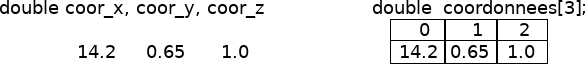
\includegraphics[width=\textwidth]{images/tableau}
\end{frame}

\begin{frame}[fragile]
	\frametitle{Propriétés des tableaux statiques}
	Les tableaux statiques sont caractérisés par deux propriétés\,:
	\begin{itemize}
		\item Le \textbf{type} de leurs éléments,
		\item Leur \textbf{taille} (qui est donc fixée à l'avance par une constante).
	\end{itemize}
    
    \begin{alertblock}{Conséquences}
    \begin{itemize}
    	\item Un tableau ne peut contenir des éléments que d'\textbf{un seul et même type},
        \item La taille d'un tableau statique \textbf{ne peut pas changer}.
    \end{itemize}
    \end{alertblock}
\end{frame}

\begin{frame}[fragile=singleslide]
	\frametitle{{Mise en \oe{}uvre}}
	\begin{exampleblock}{Déclaration}
		\centering
		\mintinline{cpp}{type nom_tableau[taille];}
	\end{exampleblock}
	
	\begin{exampleblock}{Initialisation}
    \begin{minted}{cpp}
		int mon_tableau[10];
		// Initialisation manuelle à l'aide d'une boucle
		for(int i=0; i < 10; i++){
        	mon_tableau[i] = 5;
		}

		// Déclaration et initialisation directe
		double tableau_reel[5] = {2, 3.2, 9.76, 6, 1000};

		// Déclaration puis initialisation directe
		bool tableau_bool[3];
		tableau_bool = {true, true, false};
    \end{minted}
	\end{exampleblock}
\end{frame}

\begin{frame}[fragile]
 	\frametitle{Comparaison avec les listes Python}
    Les tableaux en C++ sont plus proches des tableaux \texttt{numpy} que des listes Python.
    
	\begin{minipage}{0.49\linewidth}
		\begin{minted}{python}
        # Python
        tab1 = [0,0,0,0,0]
        tab1[2] = 5

        tab2 = ["test", 10, True]








        t = 6
        tab3 = [0 for i in range(t)]
        tab3.append(100)
		\end{minted}
 	\end{minipage}
 	\begin{minipage}{0.50\linewidth}
 		\begin{minted}{cpp}
        // C++
        int tab1[5] = {0,0,0,0,0};
        tab1[2] = 5

        bool tab1 = {"a", 10, True};
        // Erreur ! Tous les éléments doivent être booléens

        int t = 6
        int tab3[t]; // Erreur !

        const int t = 6;
        int tab3[t]; // OK: t constant
        tab3.append(100) // ERREUR
        // Un tableau ne change PAS de taille
 		\end{minted}
 	\end{minipage}
\end{frame}

\begin{frame}[fragile]
	\frametitle{Manipulation des tableaux}
	Si \texttt{\textbf{n}} est la taille du tableau, alors les indices vont de \texttt{\textbf{0}} à \texttt{\textbf{n-1}}.
    
    \begin{alertblock}{Attention}
    Tenter d'accéder à un élément hors de ces bornes résultera systématiquement en une erreur lors de l'exécution du programme.
    \end{alertblock}
	
    \begin{exampleblock}{Exemple}
	\begin{minted}{cpp}
const int n = 100; // Taille du tableau (constante)
char tab[n]; // Déclaration du tableau
tab[0] = 'a'; // OK
tab[10] = 'd'; // OK
tab[n-1] = 'k'; // OK
tab[n] = 'f'; // ERREUR
tab[-1] = 'z'; // ERREUR
	\end{minted}
    \end{exampleblock}
\end{frame}
	
\begin{frame}[fragile]
	\frametitle{Manipulation des tableaux}
	Les tableaux occupent de l'espace en mémoire (une case mémoire par élément du tableau, initialisé ou non). Il est donc nécessaire de les utiliser à bon escient.
	
    \begin{minipage}{0.49\linewidth}
        \begin{minted}{cpp}
        // Calcul de 2^99
        // Le tableau stocke tous les résultats temporaires
        int t[100];
        t[0] = 1;
        for(int i = 1; i < 100; i++){
            t[i] = t[i-1] * 2;
        }
        cout << t[99] << endl;
        \end{minted}
    \end{minipage}
    \begin{minipage}{0.49\linewidth}
        \begin{minted}{cpp}
        // Calcul de 2^99
        // (sans tableau)
        int r = 1;
        
        for(int i = 1; i < 100; i++){
            r *= 2;
        }
        cout << r << endl;
        \end{minted}
    \end{minipage}
\end{frame}

\section{Spécificités des tableaux}

\begin{frame}[fragile]
\frametitle{Tableaux et fonctions}

Une fonction peut manipuler un tableau dans sa signature~:

\begin{minipage}{0.47\linewidth}
\begin{minted}{cpp}

void affiche(int t[5]){
    for(int i=0; i<5; i++){
    	cout << t[i] << " ";
    }
    cout << endl;
}

\end{minted}
\end{minipage}
\hfill
\begin{minipage}{0.52\linewidth}
\begin{minted}{cpp}

void affiche(int t[], int taille){
    for(int i=0; i<taille; i++){
    	cout << t[i] << " ";
    }
    cout << endl;
}

\end{minted}
\end{minipage}

\vspace{0.3cm}
La première solution ne traite que le cas où la taille du tableau est toujours la même pour tous les tableaux à traiter. La seconde solution est à préférer car elle réutilisable avec des tableaux de différentes tailles, \textbf{en passant celle-ci en argument}.
\end{frame}

\begin{frame}[fragile]
\frametitle{Tableaux et fonctions}
\begin{alertblock}{Passage par référence}
\begin{itemize}
\item Un tableau est \textbf{toujours} implicitement passé par référence (il ne faut donc pas rajouter de \texttt{\&}).
\item Une fonction ne peut pas retourner de tableau.
\end{itemize}
\end{alertblock}

\begin{minipage}{0.45\linewidth}
\begin{minted}{cpp}
const int taille = 10;
double tab[taille];
init(tab);
affiche(tab);
// 0 0 0 0 0 0 0 0 0 0
\end{minted}
\end{minipage}
\hfill
\begin{minipage}{0.54\linewidth}
\begin{minted}{cpp}
void init(double t[], int taille){
    for(int i=0; i<taille; i++){
        t[i] = 0;
    }
}
\end{minted}
\end{minipage}
\end{frame}

\begin{frame}[fragile]
\frametitle{Copie et égalité de tableaux}
On ne peut pas copier directement des tableaux entre eux.
\begin{minted}{cpp}
int t1[4] = {1,2,3,4}, t2[4];
t2 = t1 ; // ERREUR : pas d'affectation avec le = pour les tableaux
\end{minted}

Seule solution : itérer sur les éléments.
\begin{minted}{cpp}
int t1[4] = {1,2,3,4}, t2[4];
for(int i = 0; i < 4; i++){
    t2[i] = t1[i];
}
\end{minted}
De même, pour tester l'égalité entre deux tableaux.
\end{frame}

\section{La librairie Imagine++}

\begin{frame}
\frametitle{Les modules}
La librairie Imagine++ contient des fonctions toutes prêtes pour réaliser de nombreuses opérations :
\begin{itemize}
\item \textbf{Common}\\ fonctions et classes basiques (Timer, Color\dots)
\item \textbf{LinAlg}\\ algèbre linéaire (inversion de matrices\dots)
\item \textbf{Graphics}\\ affichage (fenêtre 2D/3D, dessin\dots)
\item \textbf{Images}\\ classe Image et traitements d'image
\end{itemize}
\end{frame}

\begin{frame}[fragile]
\frametitle{Example d'un programme simple avec Imagine++}
\begin{minted}{cpp}
#include<iostream>
#include <Imagine/Graphics.h>
using namespace std;
using namespace Imagine;

int main(){
    int xc = 128, yc = 128, t = 0, rayon; // init variables
    openWindow(256, 256); // Ouverture de la fenetre
    while (true) { // Boucle principale
        rayon = 10 * cos(t/1000); // mise a jour du rayon
        fillCircle(xc, yc, rayon, RED); // Affichage du disque
        milliSleep(20); // Temporisation
        fillCircle(xc, yc, rayon, WHITE);// Effacement du disque	
        t++; // incremente le temps
    }
    endGraphics();
    return 0;
}
\end{minted}
\end{frame}

\begin{frame}[fragile]
\frametitle{Gestion des fenêtres}

Il est possible d'ouvrir et de travailler avec plusieurs fenêtres graphiques.

\begin{minipage}{0.49\linewidth}
\begin{minted}{cpp}

// Première fenêtre
openWindow(256,256);
fillCircle(128,128,50,RED); 

// Seconde fenêtre
openWindow(256,256);
fillCircle(128,128,50,BLUE); 

// Impossible de revenir dessiner dans
// la première fenêtre car
// elle n'a pas de nom

\end{minted}
\end{minipage}
\hfill
\begin{minipage}{0.49\linewidth}
\begin{minted}{cpp}

// Première fenêtre
Window window1 = openWindow(256,256);
fillCircle(128,128,50,RED); 
// Seconde fenêtre
Window window2 = openWindow(256,256);
fillCircle(128,128,50,BLUE); 

setActiveWindow(window1);
fillCircle(128,128,50,GREEN); 
setActiveWindow(window2);
fillCircle(128,128,50,BLACK);

// Fermeture d'une fenêtre
closeWindow(window1);

\end{minted}
\end{minipage}
\end{frame}

\begin{frame}
\frametitle{La documentation}

Le site du cours $\rightarrow$ Installation Imagine++ $\rightarrow$ Instructions
\begin{figure}
\centering
\url{http://imagine.enpc.fr/~monasse/Imagine++/}


\only<1>{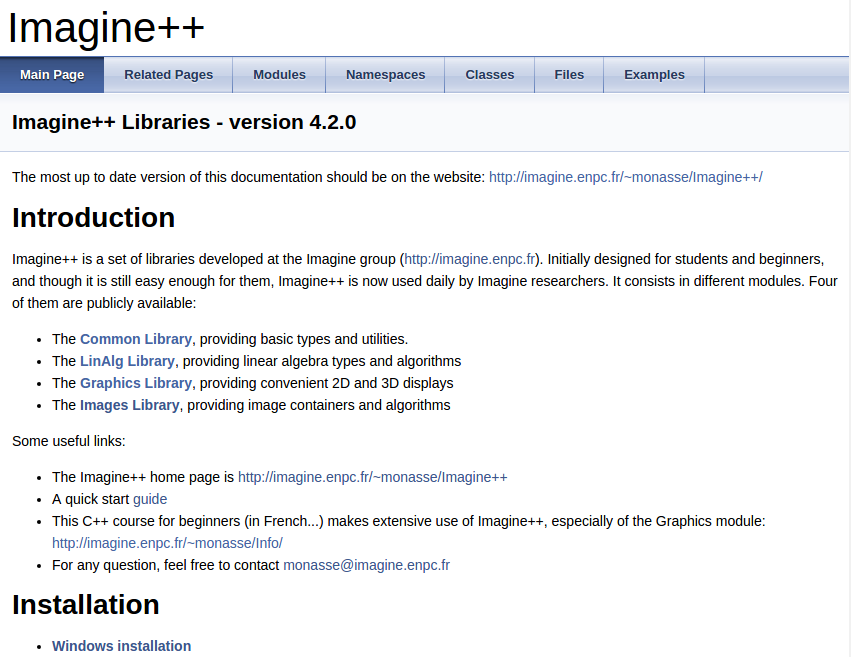
\includegraphics[width=0.7\linewidth]{images/doc_1.png}}
\only<2>{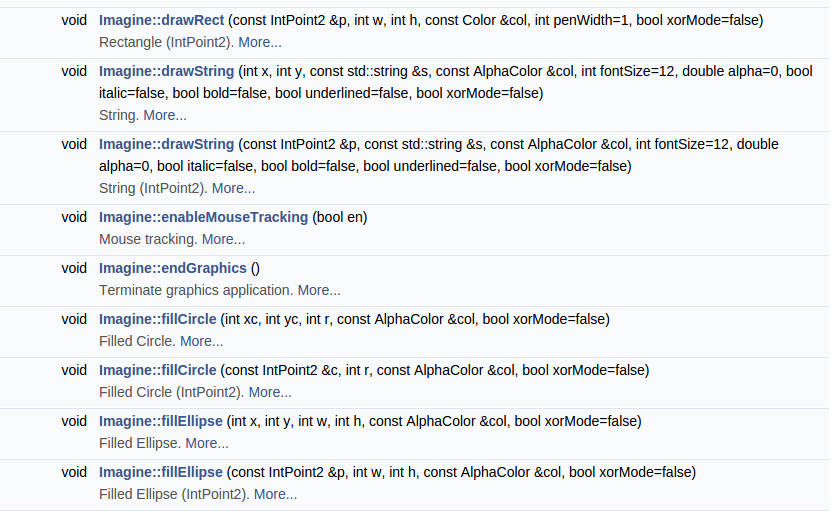
\includegraphics[width=0.7\linewidth]{images/doc_2.png}}
\only<3>{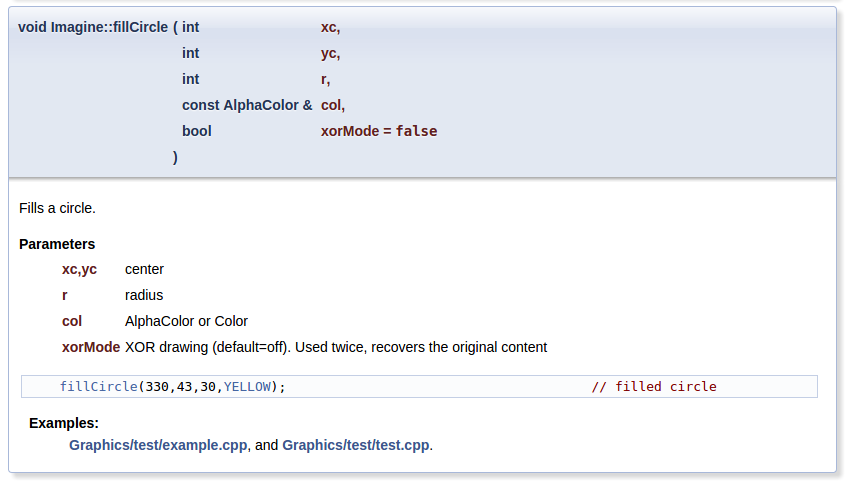
\includegraphics[width=0.7\linewidth]{images/doc_3.png}}
\end{figure}
\end{frame}

\section{TP}

\begin{frame}
\frametitle{Le TP du jour}

\begin{minipage}{0.48\linewidth}
	\begin{block}{Mastermind}
		\begin{itemize}
			\item Utilisation des tableaux
			\item Algorithmie
			\item Fonctions graphiques
		\end{itemize}
	\end{block}
    
    \begin{alertblock}{Rendu}
    À rendre \textbf{avec l'exercice individuel} au plus tard le \textbf{4/10} sur \textbf{Educnet}.
    \end{alertblock}
\end{minipage}
\hfill
\begin{minipage}{0.48\linewidth}
	\centering
	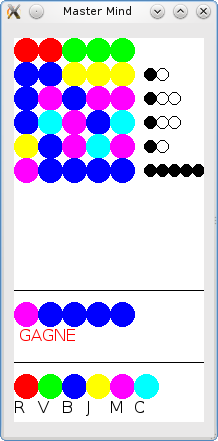
\includegraphics[width=0.6\linewidth]{images/mastermind.png}
\end{minipage}

\end{frame}

\end{document}
